% Figure: grounding tension on the level-0 ring (F=0.99, Q=0.02, sensing noise 1, channel noise 0.1).
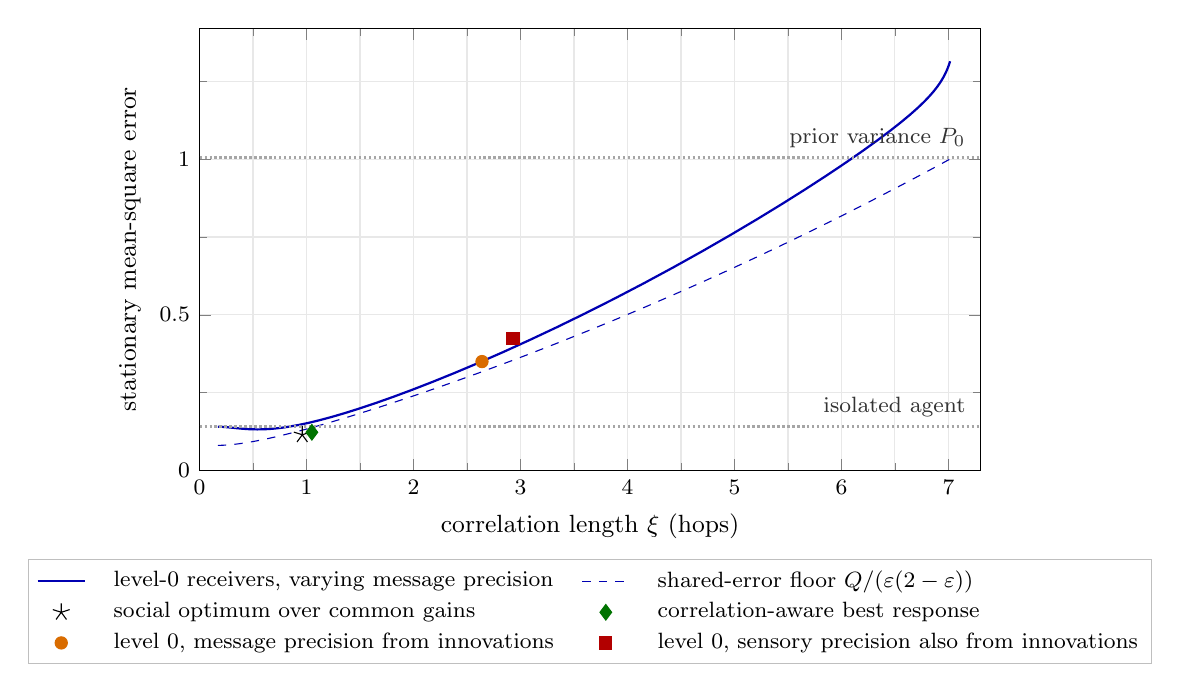
\begin{tikzpicture}
  \begin{axis}[width=11.5cm, height=7.2cm,
      xmin=0, xmax=7.3, ymin=0, ymax=1.42,
      xlabel={correlation length $\xi$ (hops)}, ylabel={stationary mean-square error},
      grid=both, grid style={gray!18}, minor tick num=1,
      legend style={font=\footnotesize, at={(0.5,-0.2)}, anchor=north, draw=gray!50, fill=white, cells={anchor=west}, legend columns=2, column sep=8pt},
      every axis label/.style={font=\small}, tick label style={font=\footnotesize}]
    \addplot[blue!70!black, thick] coordinates {(0.17121,0.14115) (0.17776,0.14107) (0.18483,0.14097) (0.19247,0.14086) (0.20074,0.14071) (0.20973,0.14054) (0.21952,0.14032) (0.23022,0.14006) (0.24194,0.13975) (0.25483,0.13937) (0.26904,0.13893) (0.28474,0.13841) (0.30216,0.13780) (0.32153,0.13712) (0.34312,0.13635) (0.36724,0.13553) (0.39425,0.13468) (0.42451,0.13385) (0.45848,0.13311) (0.49661,0.13256) (0.53941,0.13231) (0.58744,0.13252) (0.64127,0.13335) (0.70153,0.13498) (0.76886,0.13761) (0.84395,0.14143) (0.92749,0.14663) (1.02022,0.15340) (1.12287,0.16193) (1.23620,0.17238) (1.36095,0.18492) (1.49784,0.19973) (1.64754,0.21696) (1.81063,0.23679) (1.98760,0.25939) (2.17875,0.28492) (2.38415,0.31351) (2.60359,0.34528) (2.83650,0.38031) (3.08186,0.41858) (3.33819,0.46002) (3.60343,0.50444) (3.87501,0.55151) (4.14983,0.60077) (4.42437,0.65163) (4.69483,0.70337) (4.95734,0.75520) (5.20820,0.80627) (5.44414,0.85578) (5.66252,0.90301) (5.86148,0.94737) (6.04002,0.98846) (6.19794,1.02605) (6.33578,1.06010) (6.45467,1.09072) (6.55611,1.11813) (6.64184,1.14263) (6.71372,1.16456) (6.77355,1.18425) (6.82307,1.20203) (6.86385,1.21817) (6.89729,1.23292) (6.92463,1.24646) (6.94690,1.25892) (6.96501,1.27038) (6.97971,1.28090) (6.99162,1.29050) (7.00126,1.29919) (7.00905,1.30700) (7.01534,1.31394)};
    \addlegendentry{level-0 receivers, varying message precision}
    \addplot[blue!70!black, dashed] coordinates {(0.17121,0.08093) (0.17776,0.08099) (0.18483,0.08105) (0.19247,0.08113) (0.20074,0.08123) (0.20973,0.08136) (0.21952,0.08152) (0.23022,0.08171) (0.24194,0.08195) (0.25483,0.08224) (0.26904,0.08261) (0.28474,0.08306) (0.30216,0.08361) (0.32153,0.08430) (0.34312,0.08514) (0.36724,0.08618) (0.39425,0.08744) (0.42451,0.08898) (0.45848,0.09085) (0.49661,0.09312) (0.53941,0.09585) (0.58744,0.09912) (0.64127,0.10302) (0.70153,0.10764) (0.76886,0.11308) (0.84395,0.11945) (0.92749,0.12685) (1.02022,0.13541) (1.12287,0.14525) (1.23620,0.15650) (1.36095,0.16927) (1.49784,0.18372) (1.64754,0.19997) (1.81063,0.21816) (1.98760,0.23842) (2.17875,0.26088) (2.38415,0.28563) (2.60359,0.31276) (2.83650,0.34231) (3.08186,0.37425) (3.33819,0.40850) (3.60343,0.44488) (3.87501,0.48312) (4.14983,0.52284) (4.42437,0.56355) (4.69483,0.60467) (4.95734,0.64555) (5.20820,0.68551) (5.44414,0.72391) (5.66252,0.76016) (5.86148,0.79377) (6.04002,0.82442) (6.19794,0.85192) (6.33578,0.87622) (6.45467,0.89740) (6.55611,0.91564) (6.64184,0.93117) (6.71372,0.94428) (6.77355,0.95524) (6.82307,0.96436) (6.86385,0.97190) (6.89729,0.97810) (6.92463,0.98318) (6.94690,0.98732) (6.96501,0.99070) (6.97971,0.99344) (6.99162,0.99567) (7.00126,0.99747) (7.00905,0.99893) (7.01534,1.00011)};
    \addlegendentry{shared-error floor $Q/(\varepsilon(2-\varepsilon))$}
    \addplot[only marks, mark=star, mark size=3.2pt, black] coordinates {(0.96,0.115)};
    \addlegendentry{social optimum over common gains}
    \addplot[only marks, mark=diamond*, mark size=2.8pt, green!45!black] coordinates {(1.05,0.123)};
    \addlegendentry{correlation-aware best response}
    \addplot[only marks, mark=*, mark size=2.2pt, orange!85!black] coordinates {(2.64,0.350)};
    \addlegendentry{level 0, message precision from innovations}
    \addplot[only marks, mark=square*, mark size=2.2pt, red!70!black] coordinates {(2.93,0.425)};
    \addlegendentry{level 0, sensory precision also from innovations}
    \draw[gray!70, densely dotted, thick] (axis cs:0,1.005) -- (axis cs:7.3,1.005);
    \node[font=\footnotesize, gray!40!black, anchor=south east] at (axis cs:7.25,1.005) {prior variance $P_0$};
    \draw[gray!70, densely dotted, thick] (axis cs:0,0.1415) -- (axis cs:7.3,0.1415);
    \node[font=\footnotesize, gray!40!black, anchor=south east] at (axis cs:7.25,0.1415) {isolated agent};
  \end{axis}
\end{tikzpicture}
